\chapter{Pipeline Shell}
\label{ch:PipelineShell}


The Pipeline Shell is a crucial component of the reference model, designed to simulate the timing of the processor's pipeline. It interacts with the \acrfull{iss}, controlling its execution and correctly timing the output state changes. The pipeline shell also handles asynchronous events like interrupts and debug requests, determining when they can be taken and how the pipeline's state affects this.

This chapter will explore the pipeline shell's design and implementation details. We will discuss its requirements, overall architecture, and interaction with the ISS. We will also explore the different approaches for modeling the pipeline stages and controller module and how they handle instruction stepping, interrupts, side effects, flushing, and state reversion.


\section{Pipeline Shell Requirements}

The following list contains the requirements for the pipeline shell to correctly fit into the reference model design proposed in \Cref{ch:design}. The requirements are referred to as PS requirement X in the previous chapters.
In this chapter, the requirements will guide the design choices of the pipeline shell.
The pipeline shell should:
\begin{enumerate}

\item \textbf{Take RVFI data from the ISS as input} \label[psReq]{psReq:rvfiIn}
\par The pipeline shell must receive \acrshort{rvfi} data from the ISS after it has executed an instruction.

\item \textbf{Output state information through RVFI at instruction retirements} \label[psReq]{psReq:rvfiOut}
\par For the testbench to compare the reference model with the DUT core, it must output the state changes as RVFI when instructions are retired.

\item \textbf{Take in asynchronous events as inputs, independently of the core} \label[psReq]{psReq:async_input}
\par We need the pipeline shell to avoid asynchronous events depending on the core. The pipeline shell must take asynchronous events like interrupts and debug requests as inputs, independently of the core, to avoid the verification gap from \Cref{sec:back_issProblem}.



\item \textbf{Control the ISS, including when it should execute instructions and take asynchronous events} \label[psReq]{psReq:ISS-control}
\par Since the ISS should be purely functional and not responsible for the timing, the pipeline shell must control when the ISS should execute instructions and take asynchronous events.



\item \textbf{Determine when to take asynchronous events} \label[psReq]{psReq:async_control}
\par The pipeline shell should internally decide when to take asynchronous events using the pipeline state. This timing should exactly match the timing in the core.

\item \label[psReq]{psReq:side-effects} \textbf{Accurately time side effects affecting the timing of asynchronous events} 

\par Some instructions have side effects that can influence the timing of asynchronous events. The pipeline shell must accurately model the timing of these side effects to ensure the correct timing of asynchronous events.



\item \textbf{Accurately simulate pipeline details necessary to time asynchronous events} \label[psReq]{psReq:pipeline}
\par The timing of asynchronous events is influenced by various pipeline details. The pipeline shell must accurately model details like flushing and pipeline movement to ensure that the timing of asynchronous events matches the core.


%\item \textbf{The pipeline shell should be the only core-dependent component} \label[psReq]{psReq:core-dependent}
%\par 


\item \textbf{Be synthesizable and compatible with formal verification} \label[psReq]{psReq:formal}
\par To support formal verification, the pipeline shell should be designed using synthesizable \acrshort{rtl} code to ensure compatibility with formal verification tools.


\end{enumerate}


%To develop the pipeline shell, we use the following strategy:
%\begin{enumerate}
%    \item Model simple sequential pipeline that passes synchronous tests
%    \item Handle interrupts correctly in situations where interrupts can be taken immediately
%    \item Correctly model each of the signals in \sv{interrupt_allowed} to properly time interrupts in instances when they can not be taken immediately
%    \item Correctly move the instructions through the pipeline so the signals in \sv{interrupt_allowed} are properly timed
%\end{enumerate}



\section{General architecture}

As discussed in \Cref{ch:design}, the pipeline shell should control the functional ISS and correctly time the output state changes from the ISS. It should take the RVFI outputs from the ISS (\Cref{psReq:rvfiIn}), simulate how this travels through a pipeline, and output RVFI on retirements (\Cref{psReq:rvfiOut}).

\subsection{Pipeline Shell Design}

The specialization project compared two pipeline shell designs in \Cref{sec:pw_pipelineShellDesign}. It compared a \textit{stage-based pipeline simulation} modeled closely to an actual pipeline and a \textit{cycle-based time wheel simulation}, similar to the approach by \textcite{chiangEfficientTwolayeredCycleaccurate2009}. 
It concluded that a stage-based design could be easier to implement since the cycle-based approach would be complicated with pipeline flushing. However, the stage-based design could increase the probability of implementing the same bugs in the pipeline shell as in the core.


When considering a pipeline shell compatible with formal verification (\Cref{psReq:formal}), even more disadvantages with a cycle-based approach are uncovered. 
Since the \textit{time wheel} must have one stage for every cycle that an instruction is in the pipeline, the time wheel must have a dynamic size. This is problematic because dynamic arrays in SystemVerilog are not synthesizable~\cite{mehtaIntroductionSystemVerilog2021}, and therefore not compatible with formal verification~\cite{seligmanFormalVerificationEssential2015}.

%The cycle-based approach proposed by \textcite{chiangEfficientTwolayeredCycleaccurate2009} is written in SystemC. 

We choose to implement a stage-based pipeline shell with an architecture shown in \Cref{fig:pipeline_shell}. This shows how the \acrshort{if}, \acrshort{id}, \acrshort{ex}, and \acrshort{wb} pipeline stages of the CV32E40S core are modeled in the pipeline shell. 

The controller module manages the movement of instructions through the pipeline and the timing of asynchronous events. It contains the most core-specific functionality, and the pipeline stages are kept relatively simple. 


\begin{figure}
    \centering
    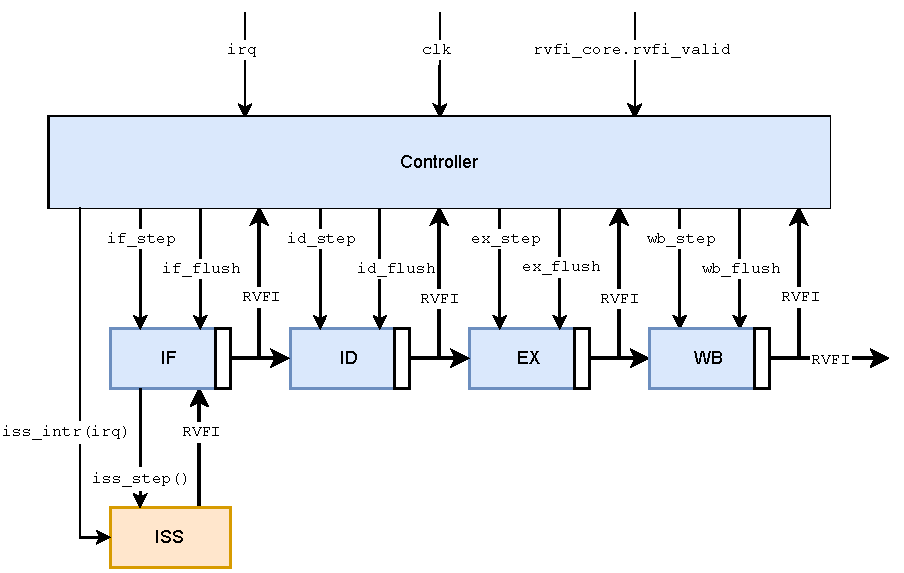
\includegraphics[width=0.75\linewidth]{figures/Pipeline_shell.pdf}
    \caption{Architecture of pipeline shell}
    \label{fig:pipeline_shell}
\end{figure}


The figure also shows that we interact with the ISS from the IF stage, where we step the ISS and get RVFI in return (\Cref{psReq:rvfiIn}). This choice comes from the discussion in \Cref{sec:pw_partition}, describing how making only one call from IF to the ISS per instruction is beneficial. 

Calling the ISS from the IF stage offers a key advantage: all information about an instruction's execution is available as it progresses through the pipeline, simplifying the design compared to calling the ISS from the WB stage. If the ISS is called from the WB stage, we do not have any information about the instructions before the WB stage. Since the controller depends on the information in the pipeline stages, decoding must happen separately from the main call to the ISS in WB. This requires splitting up the ISS call to separate fetching and decoding from the execution and writeback part. Additionally, branches and jumps need to be handled outside the ISS to keep the contents of the pipeline stages accurate. This would be complicated as a branch might depend on a register value, which again might require forwarding and execution to be implemented.

To avoid the added complexity of calling the ISS from the WB stage, we decide to interact with the ISS from the IF stage. However, this has multiple downsides that will be discussed later, requiring reversion of the ISS state on pipeline flushes (\Cref{sec:ps_revertion}) and timing of side effects (\Cref{sec:ps_side-effects}).
%
%\subsection{Compartementalizing core-specific functionality}
%
%The pipeline shell should contain the core-specific timing implementation and be adaptable to different cores. To make it easy to configure for new cores, we should also compartmentalize the core-specific details of the pipeline shell so necessary modifications for a new core are kept to a minimum.
%


\section{Dependency of core}
\label{sec:ps_dependency}

We introduce the two following possible choices for how instructions can move through the pipeline shell: 

\begin{enumerate}
    \item \textbf{Retirement-dependent pipeline shell}
    \par In this approach, instructions are moved through the pipeline stages based on instruction retirements from the core. Each time an instruction is retired, the instructions still in the pipeline are moved one stage forward. This is similar to a \textit{step-and-compare} approach from \Cref{sec:bg_verificationTech} where the ISS steps through an instruction when an instruction retires from the core. This allows the core and reference model to easily stay in sync without exactly mirroring the cycle-accurate execution of the core and is relatively simple to implement.

    \item \textbf{Core-independent pipeline shell}
    \par In this approach, the execution would be entirely independent of the core, and the movement of instructions through the pipeline would be completely contained in the pipeline shell. This complicates the pipeline shell because it has to mirror the exact execution of the core at every cycle without being concocted to the core. It must account for forwarding hazards and stalls, the exact cycle delay for \acrshort{lsu} operations, and the exact cycle count of multi-cycle instructions.
    

%Instructions can be moved through the pipeline, mirroring the functionality of the core. Every clock, each stage reports if it is ready to receive new data and if each stage has valid data ready, and the pipeline uses this to move the data through the pipeline. Additionally, signals for pending interrupts, jumps, branches, exceptions, multi-cycle instructions in progress, etc. must be considered. 


\end{enumerate}
%\tmp{40s security feature}

%\subsection{Comparison}
The CV32E40S user manual contains a table with the number of clock cycles for every multi-cycle instruction \cite{openhwgroupPipelineDetailsCOREV2023}. To implement the core-independent approach, we can use this table to determine how long an instruction should take in each stage. However, this approach can be complicated as we need specific cases for every instruction, and some instruction types have different clock cycles for different situations. Additionally, this can quickly become a complicated solution with a high probability of implementing the same bugs as the core, or other bugs.

%\begin{table}[htb]
%\centering
%\caption{Comparison of retirement and clock driven pipeline}
%\label{tab:retirementvsclock}
%\begin{tabularx}{\textwidth}{|p{15mm}|*{2}{>{\arraybackslash} X |}}
%\hline
% & Advantages & Disadvantages \\
%\hline
%Retirement dependent
%& \begin{itemize}
%\item Simpler to model
%\item Lower chance of implementing bugs from the core
%\end{itemize}
%& \begin{itemize}
%\item Does not test if instructions retire after the right amount of cycles (Not that important?)
%\item Add specific stall cases instead of movement cases
%\item Will not be equal at every clock cycle
%\item 
%\end{itemize} \\
%\hline
%Core independent
%& \begin{itemize}
%\item Cycle-accurate equal to core
%\item Can be used to verify that the core uses the correct amount of cycles for each instruction. 
%\end{itemize}
%& \begin{itemize}
%\item Hard to implement. Essentially all timing-related implementations must be implemented in the core
%\item We must calculate the cycle count for all instructions and edge cases.
%\end{itemize} \\
%\hline
%\end{tabularx}
%\end{table}

%As discussed in \Cref{sec:des_retireOrClock}, we will only compare the state after each retirement, but cycle-accurate details influences this as explained in \ref{}\tmp{TODO}.

Since we only compare the core and reference model at instruction retirements (\Cref{sec:des_retireOrClock}), it might be sufficient with a retirement-dependent pipeline shell. If this works, it would be easier to implement and less complicated. 

We choose to implement the retirement-dependent pipeline shell to determine if this simpler approach is sufficient for our needs. By implementing the simpler approach first, we can use this to implement the rest of the reference model. If the retirement-dependent approach is insufficient, we can explore the core-independent approach in future work.




\section{Pipeline Stage Modeling }%: \Cref{psReq:rvfiIn}, \ref{psReq:pipeline}, \& \ref{psReq:rvfiOut}}

This section will cover the design choices for modeling the pipeline stages within the pipeline shell. 
We want most of the core-specific timing details to be contained in the controller module. To limit the necessary modifications to a new core, we want to keep the actual pipeline stages as simple as possible. 
The goal is to strike a balance between accurately modeling the pipeline behaviour and simplifying modification to new processor cores.

\subsection{Pipeline Stage Register Content}

The pipeline shell receives an RVFI struct from the ISS after each instruction execution (\Cref{psReq:rvfiIn}). This \sv{st_rvfi} struct, along with a \sv{valid} signal, is stored in the \sv{pipe_stage_t} struct, which is passed through the pipeline. The \sv{valid} signal indicates whether the instruction is executed correctly in the ISS and is used to control the instruction flow through the pipeline.

\begin{systemverilog}
typedef struct packed {
    st_rvfi rvfi;
    logic valid;
} pipe_stage_t; 
\end{systemverilog}

When this struct reaches the \acrshort{wb} stage and has been retired, we must output RVFI from the model (\Cref{psReq:rvfiOut}). Since we use instruction retirements to control the pipeline flow, we use the \sv{valid} signal from \sv{pipe_stage_t}, in combination with the \sv{rvfi_valid} signal, to determine when the RVFI data from the struct is output and valid from the core.
%Since we use instruction retirements from the core to move through the pipeline stages, we also need to use this to output RVFI. To make sure each instruction is only marked as valid for one cycle when outputting rvfi, we need to combine the valid signal from the core, with the valid signal from the pipeline shell. This allows the RVFI output to be in sync with the core, while also only outputting RVFI when the instruction in the pipeline shell is actually valid.

%To add signals like \lstinline{rvfi_valid} we create a new interface called \lstinline{rvfi_if_t} that is passed from the pipeline shell to the reference model wrapper. 


%The WB stage therefore looks like this.
%\begin{systemverilog}
%always_ff @(posedge clk) begin
%    if (flush_i) begin
%        pipe_o.rvfi <= '0;
%        pipe_o.valid <= 1'b0;
%    end else if(step) begin
%        pipe_o.rvfi <= pipe_i.rvfi;
%        pipe_o.valid <= pipe_i.valid;
%    end
%    else begin
%        pipe_o.rvfi <= pipe_o.rvfi;
%        pipe_o.valid <= 1'b0; //Only output valid at first valid clock cycle
%    end
%end
%\end{systemverilog}



\subsection{Pipeline Stages}
Since different processor cores can have varying numbers of pipeline stages, the pipeline shell should be easily adaptable to different pipeline architectures. One option is to make a generic pipeline module with a parameterized number of equal pipeline stages. 

However, while the different pipeline stages can be fairly similar, there are some differences. Looking at \Cref{fig:pipeline_shell}, the IF stage must communicate with the pipeline, and the WB stage must correctly output RVFI from the pipeline shell. Using such a generalized design might also make implementing non-standard pipelines and out-of-order designs difficult.

Instead, we choose to create separate pipeline stage modules for each stage. This may increase the amount of modification needed to implement a new core but allows for more flexibility in implementing different types of pipelines.



\section{Controller Module Design}

The controller is the heart of the pipeline shell and is responsible for controlling the movement of instructions and the timing of asynchronous events. From \Cref{fig:pipeline_shell}, we see that it takes in the \sv{clk}, \sv{rvfi_valid} signal from the core, and asynchronous events like \sv{irq}, and \sv{debug_req} (\Cref{psReq:async_input}). It also takes in the \sv{RVFI} signals from each pipeline stage. It controls each pipeline stage with \sv{step} and \sv{flush} signals and injects asynchronous events into the ISS.

The primary functionality of the controller module includes:
\begin{enumerate}
    \item \textbf{Instruction Stepping} 
    \par The controller should determine when to execute instructions in the ISS and move instructions through the pipeline stages (\Cref{psReq:ISS-control}).
    
    \item \textbf{Asynchronous Event Handling}
    \par The controller should decide when to take asynchronous events, considering the pipeline state (\Cref{psReq:async_control}).

    \item \textbf{Timing of Side Effects} 
    \par The controller should accurately model time side effects that affect the timing of asynchronous events (\Cref{psReq:side-effects}).
    
    \item \textbf{Pipeline Flushing and State Revertion}
    \par The controller should manage the flushing of the pipeline stages caused by interrupts and branching. As will be discussed in \Cref{sec:iss_revert}, this also requires reversion of the ISS state (\Cref{psReq:pipeline}).
\end{enumerate}

The following sections will cover the design and implementation of each of these functionalities. 

%\subsubsection{Input signals}
%\begin{itemize}
%    \item \sv{clk}
%    \item \sv{rst}
%    \item \sv{valid} (Retirement from the core)
%    \item \sv{irq_i} 
%    \item \sv{if_id_pipe_i}
%    \item \sv{id_ex_pipe_i}
%    \item \sv{ex_wb_pipe_i} 
%    \item \sv{wb_pipe_i}
%    \item \sv{interrupt_allowed_i} interrupt allowed from the core
%    \item \sv{mstatus.mie} from the ISS
%\end{itemize}
%
%\subsubsection{Output signals}
%\begin{itemize}
%    \item \sv{\{if,id,ex,wb\}_step_o}
%    \item \sv{\{if,id,ex,wb\}_flush_o}
%    \item \sv{interrupt_allowed_o}
%\end{itemize}

\section{Instruction Stepping}% : \Cref{psReq:ISS-control}}

In the context of our reference model, the term \textit{step} can be used for the following actions: 
\begin{itemize}
    \item The execution of a single instruction in the ISS.
    \item The advancement of an instruction from one pipeline stage to the next.
\end{itemize}

To model a retirement-dependent pipeline, we want both actions to occur simultaneously, stepping the pipeline and loading a new instruction from the ISS into it.

In a standard pipeline, the movement of instructions in the pipeline is controlled by a \sv{ready} and a \sv{valid} signal in each pipeline stage. When both the previous stage has \sv{valid} data, and the next stage is \sv{ready} to receive new data, the instruction data is moved into the following pipeline register.

To simplify the pipeline design, we instead use a \sv{step} signal to both step the ISS and step the pipeline.
Since we use a retirement-dependent approach, the \sv{step} depends on the \sv{rvfi_valid} from the core, indicating that the core has retired an instruction. This signal is fed to all the pipeline stages as shown in \Cref{fig:pipeline_shell} and is used to step the ISS from the IF stage using the \sv{iss_step()} function.

\subsection{Halting}

In a standard pipeline, each stage can be halted, preventing instructions from moving to the next stage \cite{pattersonComputerOrganizationDesign2021}. This typically depends on the \sv{ready} and \sv{valid} signals. In our design, halting is implicitly supported since instructions will not progress in the pipeline when \sv{step} is low.

\subsection{Filling the Pipeline}

The pipeline stages are empty at the start of a simulation or after the pipeline is flushed. If we wait for the first retirement from the core before executing any instructions in the reference model, the retired instruction would only be in the IF stage of the reference model, and the execution would lag behind the core. To prevent this, the pipeline shell should proactively fill up the pipeline until all the pipeline stages contain valid instructions, and a retirement from the core would also lead to a retirement from the pipeline shell.

To implement this functionality, we use a \sv{pipe_count} counter to keep track of the amount of valid instructions in the pipeline. It initializes to 0 and increments with each step until it reaches the number of pipeline stages. When a flush occurs, it is reset to 0. Using this counter, we can force the \sv{step} signal to be high when the number is less than the number of pipeline stages, allowing the pipeline to be filled up. Once the pipeline is full, the \sv{step} is controlled by the \sv{rvfi_valid} signal from the core.

\section{Interrupt}% : \Cref{psReq:ISS-control}}
\label{sec:ps_interrupt}

This section will cover how interrupts are handled in the pipeline shell.
From here, we will use interrupts as an example of how asynchronous events can be handled in the pipeline shell. However, we will discuss how the design choices for interrupts can transfer to other asynchronous events in \Cref{sec:other_async}.


\subsection{Partitioning of Interrupt Handling Between the ISS and Pipeline Shell}

We must decide the partitioning of the interrupt handling between the ISS and the pipeline shell, choosing where the decision to take the interrupt should be made.

From \Cref{fig:interrupt_timing}, we see that the decision of taking an interrupt is divided into the \sv{pending_interrupt} and \sv{interrupt_allowed} signals, where:
\begin{itemize}
    \item \textbf{Pending Interrupt} decides whether the interrupt is pending and enabled. It depends on the incoming \sv{irq} interrupt input and \acrshort{csr}s like \rv{mie} and \rv{mstatus} to decide if the incoming interrupt is enabled.
    \item \textbf{Interrupt Allowed} determines if the pipeline is in a state where it can safely be flushed and the interrupt can be safely taken.
\end{itemize}

Since the CSRs are contained inside the ISS, and the pipeline state is contained in the pipeline shell, we choose to separate the interrupt handling so that the ISS will handle the \sv{pending_interrupt} signal, and the pipeline shell will handle the \sv{interrupt_allowed} signal. This limits the number of signals sent into the ISS to determine \sv{interrupt_allowed} and the number of signals sent out of the ISS for the pipeline shell to handle the \sv{pending_interrupt} signal.

However, when considering the timing of side effects in \Cref{sec:ps_side-effects}, this partitioning gets more complicated and might not be the best solution in hindsight. This will be discussed in \Cref{sec:dis_async_partition}.

%Implementing the \sv{interrupt_allowed} signal in the pipeline shell will be covered further in \Cref{sec:interrupt_allowed}.


When multiple interrupts are enabled, the ISS must also determine which interrupt to take. The RISC-V specification \cite{watermanRISCVInstructionSet2021} only specifies the priority of the standard interrupts (bit \rv{15:0} in \rv{mip}), while the priority of custom interrupts (\rv{31:16}) is implementation specific.

We let the ISS choose which interrupt to take, although this requires some core-specific modifications to the ISS, giving us \Cref{issReq:interruptOrdering}. We choose this approach since determining interrupt taking in the pipeline shell would require larger modifications to how interrupts are handled inside the ISS and the communication between the pipeline shell and the ISS.

%On the other hand, determining the interrupt ordering in the pipeline shell causes some problems with the communication with the ISS. Instead of injecting the bits to be set in \rv{mip} and letting the ISS operate close to its original implementation, larger modifications to interrupt handling are required. If we want to tell the ISS which interrupt to take, the ISS must be modified to take the input interrupt instead of analyzing \rv{mip} and deciding the interrupt. One approach to informing the ISS of the interrupt is to only set one \rv{mip} bit at a time, so the ISS has no choice. This can work, but causes a mismatch between the \rv{mip} register of the core and the reference model if this is read. Another way would be to override the ISS interrupt-taking functionality so that it takes a given input interrupt instead of relying on \rv{mip}.


\subsection{Interrupt Notification to the ISS}
\label{sec:ps_interrupt_to_iss}

To inform the ISS of potential interrupts, we use a dedicated function called \sv{iss_intr(...)}. This is called every clock cycle and takes \sv{irq} and \sv{interrupt_allowed} as inputs to let the ISS decide whether the interrupt should be taken. As will be discussed in \Cref{sec:ps_side-effects}, \sv{iss_intr(...)} must also consider the values from an external CSR.

The \sv{iss_intr()} function updates the \rv{mip} bits in the ISS CSR based on the incoming \rv{irq}, and the bits set in the \rv{mie} CSR. If the \sv{interrupt_allowed} signal is high, the ISS should choose to take the interrupt and return a boolean value indicating its decision. If interrupts are not enabled, it should still set the \rv{mip} bits, but the interrupt should not be taken. This requires that the ISS can enable or disable interrupts independently of the \rv{mip} bits and other CSRs. This requires a modification and gives us \Cref{issReq:interruptEnabled}. 

The partitioning and timing of the interrupt handling is shown in \Cref{fig:ps_interrupt_timing}. This shows how the \sv{irq} is input into the pipeline shell and input into the ISS with \sv{iss_intr()}, along with \sv{interrupt_allowed} and data from the External CSR. The ISS uses this information to decide if the interrupt should be taken. If this is chosen, the ISS changes the PC and CSRs to take the interrupt and informs the pipeline shell so it can flush the pipeline. The next time the pipeline shell steps the ISS using \sv{iss_step()}, it will start executing the interrupt handler.

\begin{figure}
    \centering
    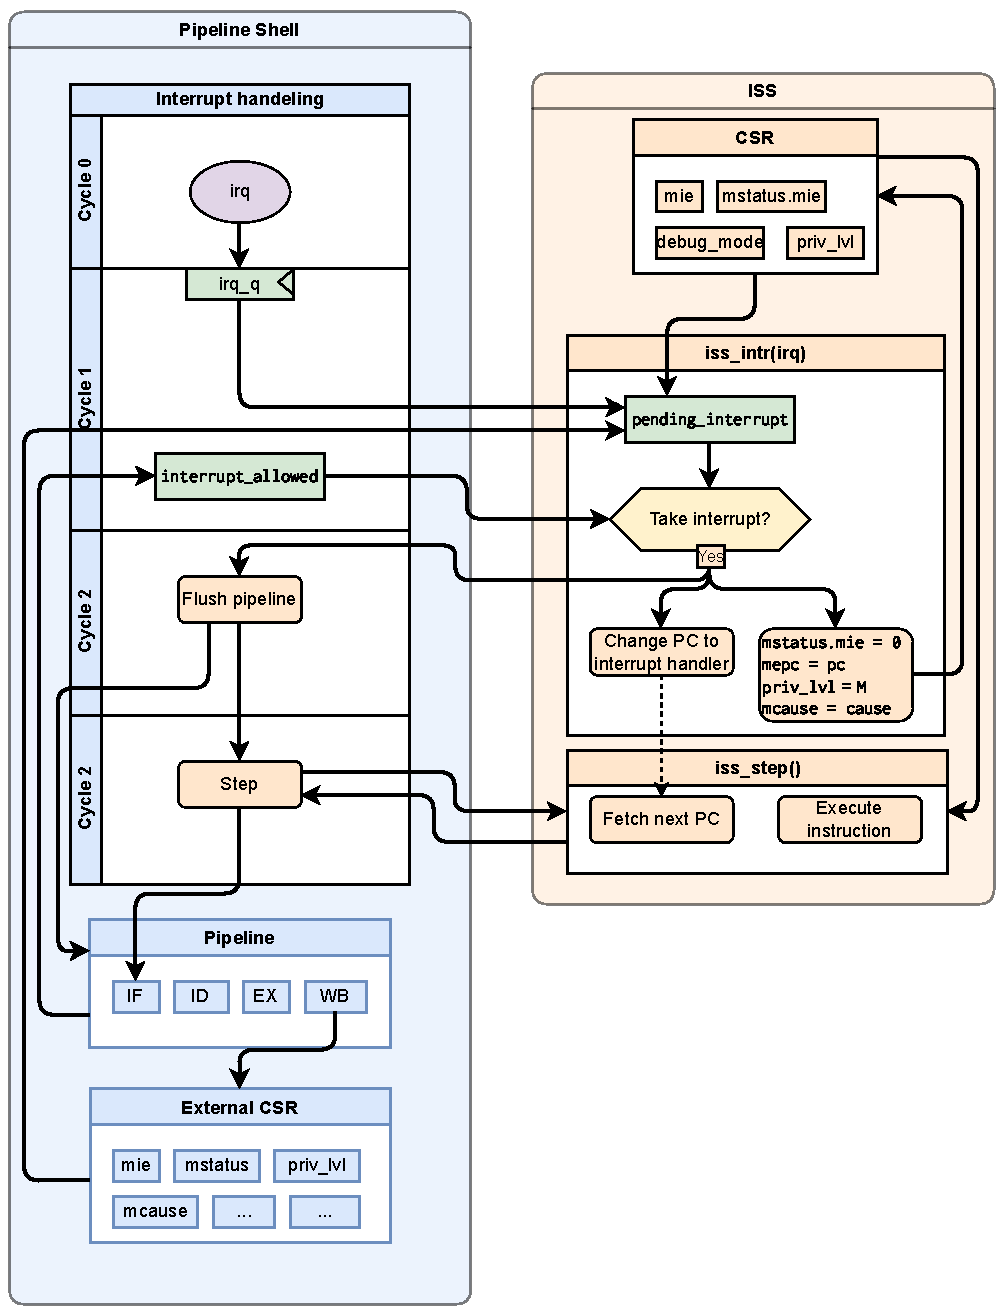
\includegraphics[width=1\linewidth]{figures/PS_interrupt_timing.pdf}
    \caption{Diagram showing the partition and timing of interrupt handling between the pipeline shell and ISS.}
    \label{fig:ps_interrupt_timing}
\end{figure}


\subsection{Interrupt Allowed}
\label{sec:interrupt_allowed}


The \sv{interrupt_allowed} signal is a critical factor in determining the timing of interrupts, indicating whether the pipeline is in a state where an interrupt can safely be taken. In the CV32E40S, the signal is influenced by various factors, including in-flight memory operations, the debug mode, multi-cycle instructions, and other pipeline-related conditions. \Cref{fig:dependency-tree-cv32x} shows the complexity of this signal and how it depends on the different pipeline stages.

Ideally, all components contributing to the \sv{interrupt_allowed} signal would be accurately modeled from the state of the pipeline shell, independently of the core. However, due to the scope of this thesis, the \sv{interrupt_allowed} signal is not modeled based on the pipeline shell but instead directly injected from the DUT core. This is done to facilitate the implementation of the other reference model components, where we can now assume that the \sv{interrupt_allowed} signal functions correctly.

Injecting the \sv{interrupt_allowed} from the core introduces a verification gap. If there is a bug in the core's implementation of this signal, the reference model will contain the same bug, leading to the bug not being detected. Therefore, future work should focus on independently modeling the \sv{interrupt_allowed} signal within the pipeline shell.

%When injecting the \sv{interupt_allowed} signal from the core and when recreating the signal, we can model the same bugs as the core. If there is a bug in implementing this signal in the core, we could end up modeling the same bug in the reference model, and the bug would not be detected. 
%%For example, if the core incorrectly allows an interrupt to be taken when there is an outstanding memory operation, the reference model could also allow the interrupt to be taken, and there would be no mismatch between the core and reference model.
%
%This reliance on the \sv{interrupt_allowed} signal is one considerate disadvantage of this implementation. It is important to be mindful of this limitation and avoid using the implementation from the core as much as possible when implementing this in the reference model.



%One disadvantage of this approach is that it leads to many more DPI function calls to the ISS, which can decrease performance.


\section{Timing Side effects}% : \Cref{psReq:side-effects}}
\label{sec:ps_side-effects}

\subsection{Side Effects Influencing Interrupt Timing}

Some side effects affect the timing of interrupts, like changes to the \rv{mie} and \rv{mstatus} CSRs. The chosen pipeline shell architecture leads to a problem with side effects, which will be explained in an example.

\begin{figure}
    \centering
    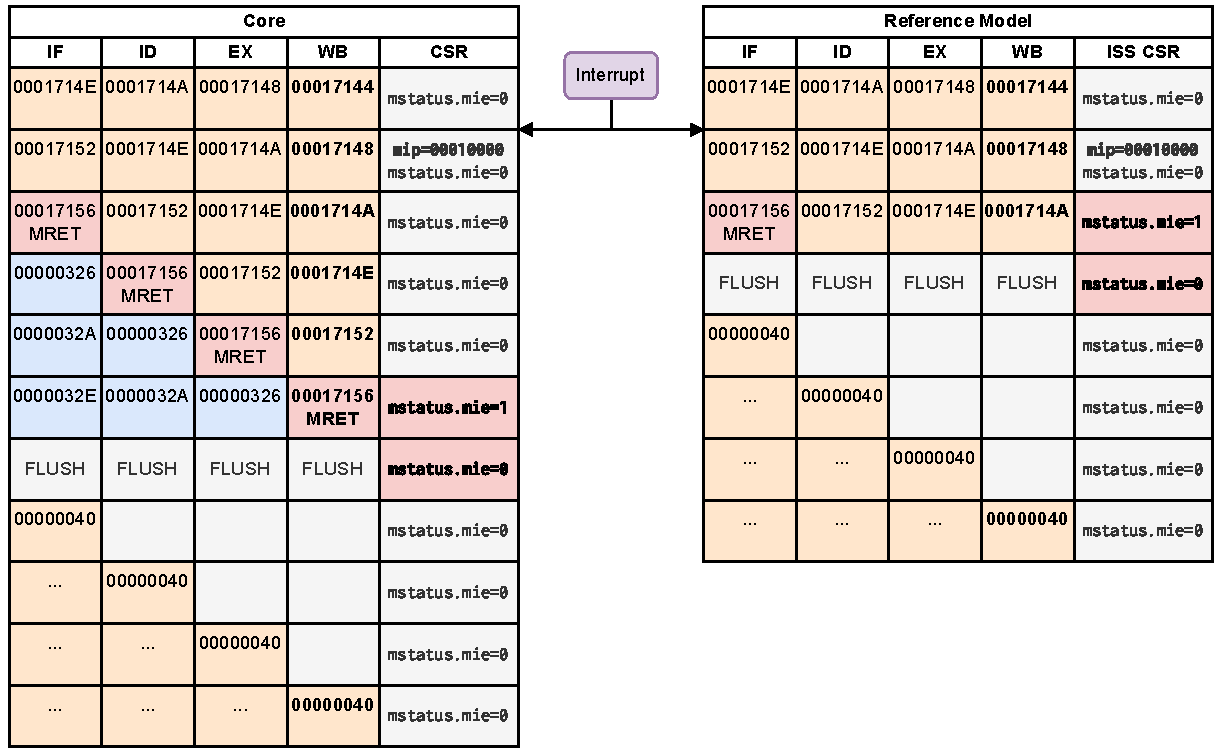
\includegraphics[width=1\linewidth]{figures/mret_example_fail.pdf}
    \caption{Example showing the mismatch of execution between the core and reference model when an interrupt is taken directly after another interrupt.}
    \label{fig:mret_example_fail}
\end{figure}


\Cref{fig:mret_example_fail} shows the the instructions in the pipelines of the CV32E40S core, and the reference model. In the example, we use the internal CSR inside the ISS to determine if interrupts are enabled. The figure also shows the CSR value of the \rv{mstatus.mie} bit in the core and the ISS CSR. The example shows the execution at the end of an interrupt handler (orange instructions) that returns to normal program flow with the \rv{mret} instruction. When executing this instruction in the WB stage, it should re-enable interrupts by setting \rv{mstatus.mie = 1}, and change the PC to the next instruction before it was interrupted. A new interrupt is injected into the core and reference model while the processor is still in an interrupt handler. Since \rv{mstatus.mie} is 0, the interrupt is not taken yet. 

In our design, the ISS executes the instructions in the IF stage. The figure shows that the ISS CSR immediately sets \rv{mstatus.mie = 1} when \rv{mret} runs in the IF stage of the reference model. This causes the pending interrupt to be taken the next cycle instead of returning to the normal execution flow (blue instructions) as the core does. This causes the instructions with PC \rv{0001714E, 00017152, and 00017156} not to be retired from the reference model before the interrupt is taken.





\subsection{External CSR}

To address this timing discrepancy, we introduce an \textit{External CSR} within the pipeline shell. It should store the CSR values that affect the interrupt timing, and should be updated as instructions progress through the pipeline. By using the values in the external CSR when evaluating interrupts, we ensure that the reference model accurately reflects the state of the CSRs at the time the interrupt is considered.

Since the ISS decides when interrupts are allowed, we must pass the relevant values from the external CSR to the ISS by adding these values to the \sv{iss_intr()} function. This requires the ISS to take external CSR values as inputs and consider these when taking an interrupt. This gives us \Cref{issReq:set_CSR}. Additionally, the ISS must be able to output the modified CSR values through RVFI, giving us \Cref{issReq:CSR_out}.
These CSR changes can then travel through the pipeline and update the external CSR when they reach the WB stage.


\Cref{fig:mret_example} shows the same example as above but using an external CSR updated when the CSR changes reach the WB stage. The value from the external CSR is considered before taking an interrupt. The example shows both the CSR from the ISS and the external CSR.

\begin{figure}
    \centering
    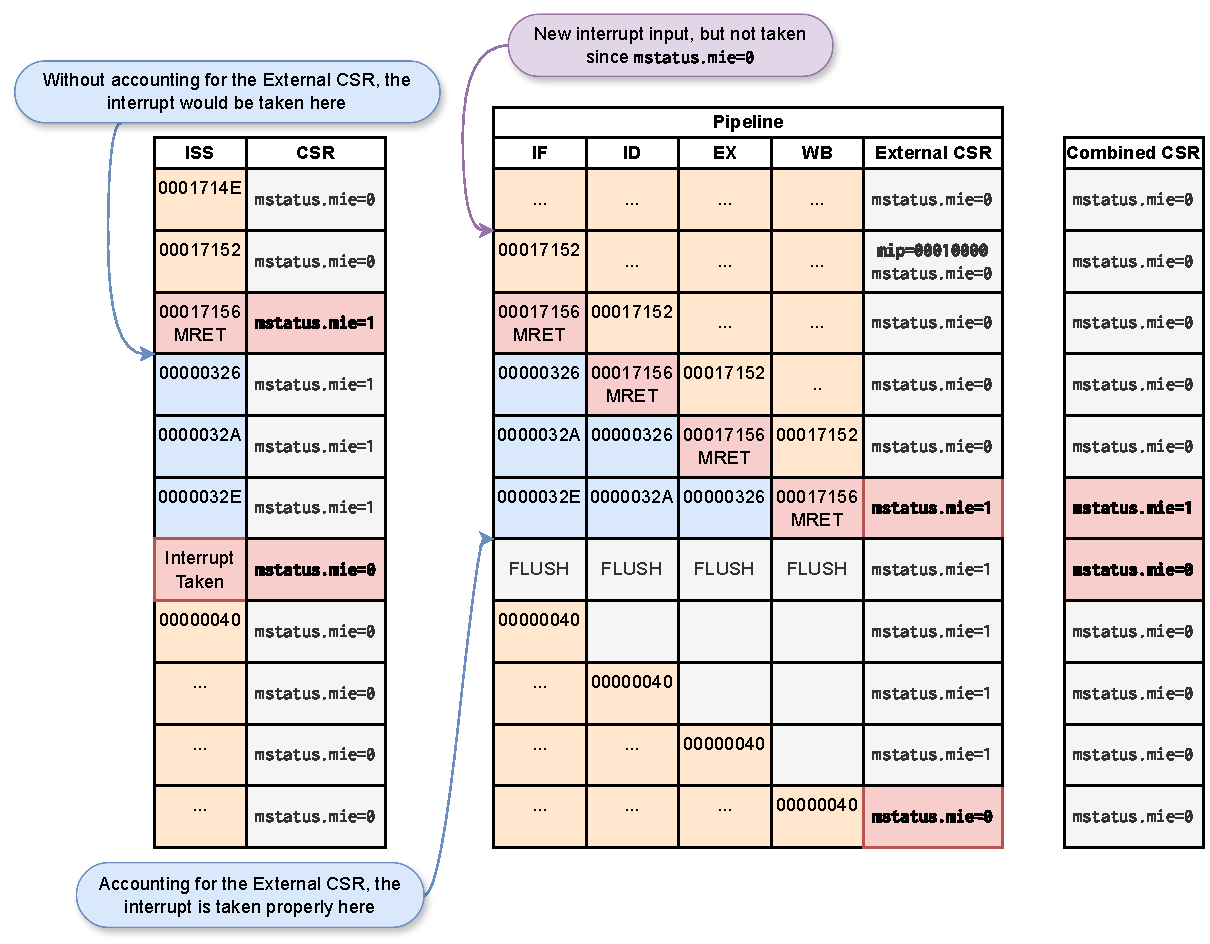
\includegraphics[width=1\linewidth]{figures/mret_example.pdf}
    \caption{Example showing how the timing of CSRs can influence interrupt timing.}
    \label{fig:mret_example}
\end{figure}

We see that in the ISS, the interrupt is not immediately taken after the \rv{mret} instruction since it also considers the external CSR, where \rv{mstatus.mie} is 0. When \rv{mret} reaches WB in the pipeline shell, the external CSR is updated, and the interrupt is taken. 

At this point, we have another problem with CSR timing. CSRs are not always updated in the WB stage. The example shows that in the external CSR, \rv{mstatus.mie} is high until the interrupt handler reaches WB. However, as seen in \Cref{fig:interrupt_timing}, the core immediately disables \rv{mstatus.mie} when an interrupt is taken.

Therefore, we define the \sv{interrupt_enabled} signal that is sent to the ISS with \sv{iss_intr()}. It should go high when \rv{mstatus.mie} reaches WB, and go low immediately after an interrupt is taken. This behavior is shown \Cref{fig:mstatus_mie}, which shows how the signal can be modeled using the \sv{wb_mstatus.mie} signal generated from the WB stage, and the \sv{interrupt_taken} returned from \sv{iss_intr()}.

\begin{figure}
    \centering
    \begin{tikztimingtable}
      \sv{clk}                  & 10{2C} G \\ 
      \sv{wb_mstatus.mie}       & LL   2{2H} 7{2L} \\ 
      \sv{interrupt_taken}      & 5{2L}  2{2H} 3{2L} \\ 
      \sv{interrupt_enabled}    & LL 6{2H} 3{2L} \\
    \end{tikztimingtable}
    \caption{Timing of \sv{interrupt_enable} and \sv{mstatus.mie}}
    \label{fig:mstatus_mie}
\end{figure}

The desired \rv{mstatus.mie} signal is shown in the combined CSR column in \Cref{fig:mret_example}, showing that \rv{mstatus.mie} is enabled when \rv{mret} reaches WB and disabled when the interrupt is taken the next cycle.

The previous example focuses on \rv{mstatus}, but the same problem can, for example, also occur immediately following a write to the \rv{mie} CSR that enables a previously disabled \rv{irq}. It can also be solved by storing \rv{mie} in the external CSR.

\section{Pipeline Flushing and ISS Revertion}

\subsection{Flushing}

As described in \Cref{sec:bg_flushing}, we must discard instructions already in the pipeline when the PC is changed by a jump, branch, or interrupt.
To model our pipeline shell, we will also need to implement pipeline flushing.

\subsubsection{Flush After Jump/Branch}

A typical pipeline flushes when the core jumps or branches to a new PC \cite{pattersonComputerOrganizationDesign2021}. Since we call the ISS in the IF stage, and the ISS fully executes one instruction before the next, the ISS always executes the correct instruction after a branch or jump, and we do not get the same incorrect instructions as the core in the pipeline that need to be flushed.

The CV32E40S core executes jumps in the ID stage and branches in the EX stage \cite{openhwgroupPipelineDetailsCOREV2023}. This means the core and reference model can mismatch the IF and ID stages before a jump or branch is correctly taken in the core. However, looking at \Cref{fig:dependency-tree-cv32x}, we see that the state of the IF is not required for interrupt timing and that the ID stage is only relevant for \acrshort{clic} interrupts. Since we, for the time being, only support \acrshort{clint} interrupts, we choose to ignore flushing the pipeline because of jumps and branches, but this assumption should be re-evaluated when implementing \acrshort{clic} interrupts in future work.


\subsubsection{Flushing After an Interrupt}

Since interrupts are asynchronous to the processor execution, we can not ignore the flushing caused by interrupts. When the interrupt is taken, the remaining instructions in the pipeline must be flushed. In our implementation, we clear the \sv{rvfi} data in each pipeline stage and set the \sv{valid} signal to 0. We use the \sv{if_flush, id_flush, ex_flush}, and \sv{wb_flush} from the controller to the pipeline stages to control flushing in each stage. When the ISS decides to take an interrupt, the \sv{iss_intr()} function returns true, and the \sv{interrupt_taken} signal is set. This signal can be output to the pipeline stages with the \sv{flush} signals.


%\begin{systemverilog}
%    assign flush_pipeline = interrupt_taken || debug_taken_q;
%
%    always_comb begin
%        if_flush_o <= flush_pipeline;
%        id_flush_o <= flush_pipeline;
%        ex_flush_o <= flush_pipeline;
%        wb_flush_o <= flush_pipeline;
%    end
%\end{systemverilog}


\section{State Revertion}
\label{sec:ps_revertion}

In a traditional pipeline, where the state changes are applied in the WB stage, flushing each pipeline stage is sufficient to discard the effects of the instruction \cite{pattersonComputerOrganizationDesign2021}.

However, in our reference model, the ISS executes an entire instruction before passing the result to the IF stage.
This means that the instruction's state changes are already applied within the ISS, and flushing the pipeline alone will not undo these changes. This is one of the significant disadvantages of calling the ISS in the IF stage compared to calling the ISS in the WB stage.

To address this and properly flush the pipeline shell, we need a mechanism to revert the state of the ISS to a previous state.
This involves restoring register values, \acrshort{csr}s, memory writes, and other relevant state information.

This is in some ways comparable to the rollback approach used by some lock-step processors \cite{marquesLockVHeterogeneousFault2021, liDuckCoreFaultTolerantProcessor2021, nikiemaDesignLowComplexity2023} to \textit{rollback} the processor context of two synced cores if they diverge. \textcite{marquesLockVHeterogeneousFault2021} saves a \textit{snapshot} of the state of the processor at various \textit{checkpoints} along the execution, and if a fault is found, the state is reverted to the previous valid checkpoint.

We can use a similar approach to store the state of the ISS into \textit{snapthots} we can revert back to. Since an interrupt and flush can happen at any instruction, we need a checkpoint between every instruction.


To properly revert the state of the ISS, we must be able to revert all possible external and state changes caused by executing an instruction. The most important registers are the 32 \acrfull{gpr} and the \acrfull{pc}, which are written to or read from at almost every instruction \cite{watermanRISCVInstructionSet2019}.
Some \acrfull{csr} are also changed because of instructions and must be stored. Many CSRs are likely to remain static like the \rv{mvendorid}, \rv{misa}, and \rv{marchid}, while others may change during execution like \rv{mstatus}, \rv{mie}, and \rv{mscratch} \cite{watermanRISCVInstructionSet2021}. Therefore, we must decide to only store some relevant CSRs or all CSRs.

Additionally, since we use the ISS's internal memory simulation, we need to revert potential memory writes that occurred for instructions that must be discarded.


\subsection{Store States in Pipeline Shell or ISS}

We can either store these states inside the ISS or in the Pipeline shell. By outputting the snapshot and moving it through the pipeline, it would theoretically be simple to input the state of the oldest instruction in the pipeline into the ISS and revert back to it. This could be more practical if a core-independent pipeline shell is chosen in \Cref{sec:ps_dependency}. In practice, converting the snapshot into SystemVerilog may be difficult, and it must be contained enough to be sent through the pipeline easily. %Another solution could be not to store the entire state as a snapshot but only store the state changes. This would require iterating through the pipeline stages in reverse and reversing all the stored state changes.

Instead, we choose to store the snapshot inside the ISS. This keeps the state contained and allows the snapshot to be stored in a logical format to the ISS without converting it to and from SystemVerilog to be sent through the pipeline. 
To revert the state from outside the ISS, we introduce a \sv{revert_steps} parameter to the \sv{iss_intr()} function. This parameter indicates the number of states to revert, allowing the ISS to revert the instructions flushed in a typical pipeline.
This gives us \Cref{issReq:revertState}, specifying that the ISS must be able to revert to a previous state, reverting registers, CSRs, and memory operations.

\subsection{When To Revert}
\label{sec:ps_when_revert}

The order of events when reverting the state is essential to get right.
The naive order could look something like this:

\begin{enumerate}
    \item An interrupt is input into the reference model
    \item The reference model decides if the interrupt is allowed and inputs the \rv{irq} bits into the ISS with \sv{iss_intr()}
    \item The ISS reports that the interrupt is taken
    \item The pipeline shell is flushed
    \item We revert the ISS to a previous state
    \item The ISS starts running the interrupt handler
\end{enumerate}

This order is problematic. When we run the \sv{iss_intr()} function and the interrupt is taken in the ISS, this sets the \rv{mepc} and \rv{mstatus} CSRs as explained in \Cref{sec:bg_interrupts}. Reverting the state after the interrupt is taken in the ISS, like above, discards these CSR writes since the CSRs are reverted to a previous state. Since interrupt taking is decided inside the ISS, we can also not revert the state before running the \sv{iss_intr()} function.

To overcome this, we must revert the state before setting the \rv{mip}, but after deciding that the interrupt will be taken. We choose to revert the state from inside the ISS, instead of using a separate \sv{iss_revert()} function from the pipeline shell. Therefore, we add a \sv{revert_steps} parameter to the \sv{iss_intr()} function so that state revertion can be done inside the ISS.

This gives us the following order:

\begin{enumerate}
    \item An interrupt is input into the reference model
    \item The reference model decides if the interrupt is allowed and inputs the \rv{irq} bits into the ISS with \sv{iss_intr()}
    \item The ISS decides the interrupt will be taken
    \item The ISS reverts the state
    \item  The ISS takes the interrupt and writes to the relevant CSRs
    \item The pipeline shell is flushed
    \item The ISS starts running the interrupt handler
\end{enumerate}

\subsection{How Many States To Revert}

\begin{figure}
    \centering
    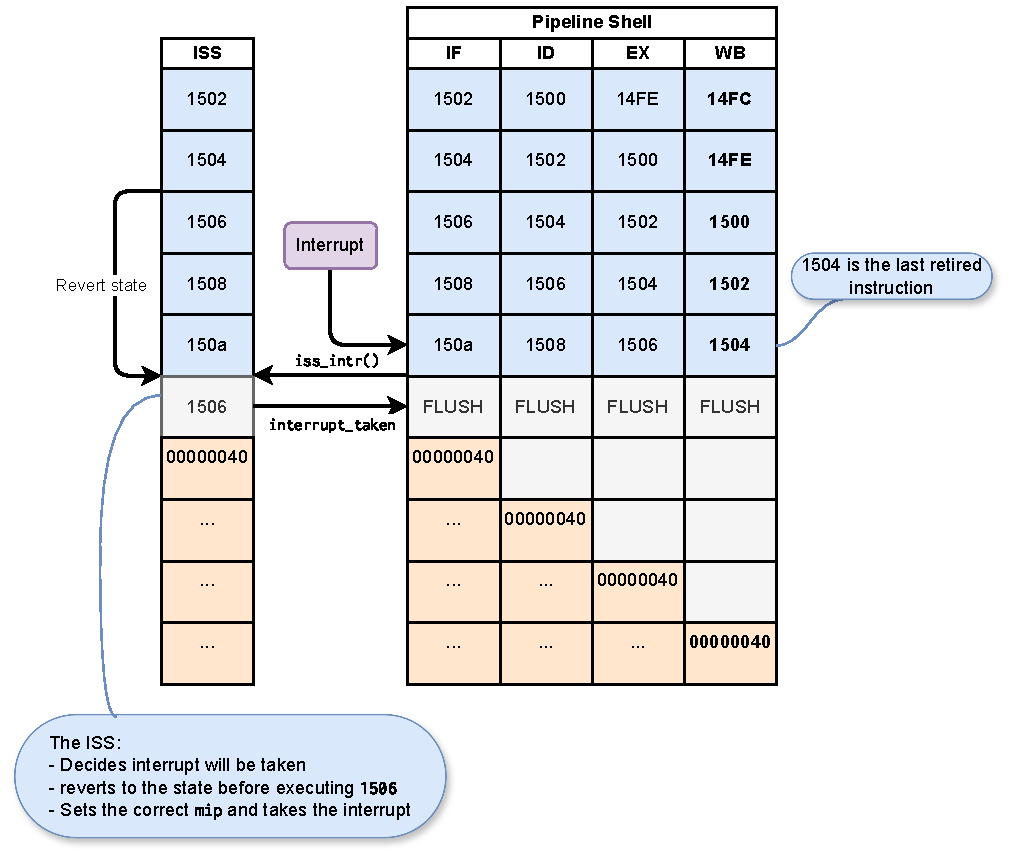
\includegraphics[width=0.85\linewidth]{figures/revert_example.pdf}
    \caption{Example showing how many instructions we need to revert the state when flushing the pipeline after.}
    \label{fig:revert_example}
\end{figure}


We can use the example in \Cref{fig:revert_example} to determine the number of steps to revert.
This shows the PC of the instructions in the pipeline shell and the PC of instructions executed in the ISS. In the WB stage, we see the retired instructions in bold, which are output over RVFI. An interrupt is applied when \sv{1504} retires, and the reference model decides that interrupts are allowed and calls the ISS with \sv{iss_intr()}. Since \sv{1504} is the last instruction to retire, we need to discard the changes from \sv{150a}, \sv{1508}, and \sv{1506} by reverting the state of the ISS to the state before it executed \sv{1506}. After the reversion is done, the ISS can take the interrupt, and \sv{1506} will be stored in the \rv{mepc} CSR and be the first instruction to run when the interrupt handler is completed.

With our current retirement-dependent implementation, we must always revert the same number of instructions for a given number of pipeline stages since we always step the ISS in conjunction with the pipeline. However, we would likely need to revert a variable number of instructions for a core-independent approach. For our implementation of the CV32E40S core with four pipeline stages, we see from the figure that we always need to revert three instructions.



%
%\begin{figure}[htb]
%\centering
%\begin{ganttchart}[
		x unit=1.4cm,
		y unit chart=0.7cm,
		canvas/.style={draw=none,fill=none}, % remove canvas borders, etc
		vgrid={*{2}{draw=black!8}},           % vertical gray lines every unit
		inline,                              % draw bars inline
		group/.style={draw=none,fill=none},  % remove group borders, etc
		bar top shift=0.1,                   % give bar 10% padding top/bottom
		bar height=0.8,                      % bar size 80% of vertical space
		y unit title=0.5cm,                  % crop titles a little smaller
		title/.style={draw=none,fill=none},  % remove title borders, etc
		include title in canvas=false        % no vertical grid in title
	]{-2}{4}

    %\gantttitlelist{Cycle,IF,ID,EX,WB}{1}

	\gantttitle{Cycle}{-1}
	\gantttitle{ISS}{3}
 
	\gantttitle{}{1}
	\gantttitle{IF}{-1}
	\gantttitle{ID}{3}
	\gantttitle{EX}{-1}
	\gantttitle{WB}{3} \\

	\ganttgroup[inline=false]{1}{0}{4}
	\ganttbar[bar/.style={draw=black!80,fill=orange!40},name=iss0 ]{1}{-2}{-2}
	\ganttbar[bar/.style={draw=black!80,fill=orange!40}  ]{1}{0}{0}\\
 
	\ganttgroup[inline=false]{2}{0}{4}
	\ganttbar[bar/.style={draw=black!80,fill=yellow!40}, name=iss1  ]{2}{-2}{-2}
	\ganttbar[bar/.style={draw=black!80,fill=yellow!40}  ]{2}{0}{0}
	\ganttbar[bar/.style={draw=black!80,fill=orange!40}  ]{1}{1}{1}\\
 
	\ganttgroup[inline=false]{3}{0}{4}
	\ganttbar[bar/.style={draw=black!80,fill=lime!40},name=iss2    ]{3}{-2}{-2}
	\ganttbar[bar/.style={draw=black!80,fill=lime!40}    ]{3}{0}{0}
	\ganttbar[bar/.style={draw=black!80,fill=yellow!40}  ]{2}{1}{1}
	\ganttbar[bar/.style={draw=black!80,fill=orange!40}  ]{1}{2}{2}\\
 
	\ganttgroup[inline=false]{4}{0}{4}
	\ganttbar[bar/.style={draw=black!80,fill=green!40},name=iss3   ]{4}{-2}{-2}
	\ganttbar[bar/.style={draw=black!80,fill=green!40}   ]{4}{0}{0}
	\ganttbar[bar/.style={draw=black!80,fill=lime!40}    ]{3}{1}{1} 
	\ganttbar[bar/.style={draw=black!80,fill=yellow!40}  ]{2}{2}{2} 
	\ganttbar[bar/.style={draw=black!80,fill=orange!40}  ]{1}{3}{3} 
	\ganttbar[bar/.style={draw=none}  ]{\textbf{valid}}{4}{4} \\
 
	\ganttgroup[inline=false]{(IRQ) 5}{0}{4}
    \ganttbar[bar/.style={draw=black!80,fill=cyan!40},name=iss4    ]{5}{-2}{-2} 
    \ganttbar[bar/.style={draw=black!80,fill=cyan!40}    ]{5}{0}{0} 
	\ganttbar[bar/.style={draw=black!80,fill=green!40}   ]{4}{1}{1}
	\ganttbar[bar/.style={draw=black!80,fill=lime!40}    ]{3}{2}{2} 
	\ganttbar[bar/.style={draw=black!80,fill=yellow!40}  ]{2}{3}{3}  
	\ganttbar[bar/.style={draw=none}  ]{\textbf{valid}}{4}{4} \\


	\ganttgroup[inline=false]{(Revert(2)) 6}{0}{1}
    \ganttbar[bar/.style={draw=black!80,fill=black!10},name=iss5    ]{3}{-2}{-2} 
    \ganttbar[bar/.style={draw=black!80,fill=black!10}    ]{}{0}{0} 
    \ganttbar[bar/.style={draw=black!80,fill=black!10}    ]{}{1}{1} 
    \ganttbar[bar/.style={draw=black!80,fill=black!10}    ]{}{2}{2} 
    \ganttbar[bar/.style={draw=black!80,fill=black!10}    ]{}{3}{3} 
    
    \\
    
	\ganttgroup[inline=false]{7}{0}{1}
	\ganttbar[bar/.style={draw=black!80,fill=red!50}]{IH1}{-2}{-2}
	\ganttbar[bar/.style={draw=black!80,fill=red!50}]{IH1}{0}{0} \\

	\ganttgroup[inline=false]{8}{0}{1}
	\ganttbar[bar/.style={draw=black!80,fill=orange!80}    ]{IH2}{-2}{-2}
	\ganttbar[bar/.style={draw=black!80,fill=orange!80}    ]{IH2}{0}{0}
	\ganttbar[bar/.style={draw=black!80,fill=red!50}       ]{IH1}{1}{1} \\
	
	\ganttgroup[inline=false]{9}{0}{1}
	\ganttbar[bar/.style={draw=black!80,fill=yellow!80}    ]{IH3}{-2}{-2}
	\ganttbar[bar/.style={draw=black!80,fill=yellow!80}    ]{IH3}{0}{0}
	\ganttbar[bar/.style={draw=black!80,fill=orange!80}    ]{IH2}{1}{1}
	\ganttbar[bar/.style={draw=black!80,fill=red!50}       ]{IH1}{2}{2} \\
 
	\ganttgroup[inline=false]{10}{0}{1}
	\ganttbar[bar/.style={draw=black!80,fill=lime}       ]{IH4}{-2}{-2}
	\ganttbar[bar/.style={draw=black!80,fill=lime}       ]{IH4}{0}{0}
	\ganttbar[bar/.style={draw=black!80,fill=yellow!80}    ]{IH3}{1}{1}
	\ganttbar[bar/.style={draw=black!80,fill=orange!80}    ]{IH2}{2}{2}
	\ganttbar[bar/.style={draw=black!80,fill=red!50}       ]{IH1}{3}{3}  
	\ganttbar[bar/.style={draw=none}  ]{\textbf{valid}}{4}{4}\\


    \ganttlink[]{iss2}{iss5}

    %\ganttlink[link type=rdldr]{[xshift=-0.3cm]iss3.east}{[yshift=1cm]iss3.east}{[yshift=1cm]iss2.east}
    %\ganttlink[]{[yshift=1cm]iss4.east}{[yshift=1cm]iss3.east}

\end{ganttchart}

%\caption{\tmp{TODO: fix figure}Illustrate state reversion with ISS content and pipeline content.}
%\label{fig:interrupt_revert_addi}
%\end{figure}
%
%\begin{figure}[htb]
%\centering
%\begin{ganttchart}[
		x unit=1.4cm,
		y unit chart=0.7cm,
		canvas/.style={draw=none,fill=none}, % remove canvas borders, etc
		vgrid={*{2}{draw=black!8}},           % vertical gray lines every unit
		inline,                              % draw bars inline
		group/.style={draw=none,fill=none},  % remove group borders, etc
		bar top shift=0.1,                   % give bar 10% padding top/bottom
		bar height=0.8,                      % bar size 80% of vertical space
		y unit title=0.5cm,                  % crop titles a little smaller
		title/.style={draw=none,fill=none},  % remove title borders, etc
		include title in canvas=false        % no vertical grid in title
	]{-2}{4}

    %\gantttitlelist{Cycle,IF,ID,EX,WB}{1}

	\gantttitle{Cycle}{-1}
	\gantttitle{ISS}{3}
 
	\gantttitle{}{1}
	\gantttitle{IF}{-1}
	\gantttitle{ID}{3}
	\gantttitle{EX}{-1}
	\gantttitle{WB}{3} \\

	\ganttgroup[inline=false]{1}{0}{4}
	\ganttbar[bar/.style={draw=black!80,fill=orange!40},name=iss0 ]{1}{-2}{-2}
	\ganttbar[bar/.style={draw=black!80,fill=orange!40}  ]{1}{0}{0}\\
 
	\ganttgroup[inline=false]{2}{0}{4}
	\ganttbar[bar/.style={draw=black!80,fill=yellow!40}, name=iss1  ]{2}{-2}{-2}
	\ganttbar[bar/.style={draw=black!80,fill=yellow!40}  ]{2}{0}{0}
	\ganttbar[bar/.style={draw=black!80,fill=orange!40}  ]{1}{1}{1}\\
 
	\ganttgroup[inline=false]{3}{0}{4}
	\ganttbar[bar/.style={draw=black!80,fill=lime!40},name=iss2    ]{3}{-2}{-2}
	\ganttbar[bar/.style={draw=black!80,fill=lime!40}    ]{3}{0}{0}
	\ganttbar[bar/.style={draw=black!80,fill=yellow!40}  ]{2}{1}{1}
	\ganttbar[bar/.style={draw=black!80,fill=orange!40}  ]{1}{2}{2}\\
 
	\ganttgroup[inline=false]{4}{0}{4}
	\ganttbar[bar/.style={draw=black!80,fill=green!40},name=iss3   ]{4}{-2}{-2}
	\ganttbar[bar/.style={draw=black!80,fill=green!40}   ]{4}{0}{0}
	\ganttbar[bar/.style={draw=black!80,fill=lime!40}    ]{3}{1}{1} 
	\ganttbar[bar/.style={draw=black!80,fill=yellow!40}  ]{2}{2}{2} 
	\ganttbar[bar/.style={draw=black!80,fill=orange!40}  ]{1}{3}{3} 
	\ganttbar[bar/.style={draw=none}  ]{\textbf{valid}}{4}{4} \\
 
	\ganttgroup[inline=false]{5}{0}{4}
    \ganttbar[bar/.style={draw=black!80,fill=cyan!40},name=iss4    ]{5}{-2}{-2} 
    \ganttbar[bar/.style={draw=black!80,fill=cyan!40}    ]{5}{0}{0} 
	\ganttbar[bar/.style={draw=black!80,fill=green!40}   ]{4}{1}{1}
	\ganttbar[bar/.style={draw=black!80,fill=lime!40}    ]{3}{2}{2} 
	\ganttbar[bar/.style={draw=black!80,fill=yellow!40}  ]{2}{3}{3}  
	\ganttbar[bar/.style={draw=none}  ]{\textbf{valid}}{4}{4} \\

	\ganttgroup[inline=false]{6}{0}{4}
    \ganttbar[bar/.style={draw=black!80,fill=cyan!40}    ]{5}{0}{0} 
	\ganttbar[bar/.style={draw=black!80,fill=green!40}   ]{4}{1}{1}
	\ganttbar[bar/.style={draw=black!80,fill=lime!40}    ]{3}{2}{2} 
	\ganttbar[bar/.style={draw=black!80,fill=yellow!40}  ]{2}{3}{3}  
	   \\

	\ganttgroup[inline=false]{(IRQ) 7}{0}{4}
    \ganttbar[bar/.style={draw=black!80,fill=cyan!40}    ]{5}{0}{0} 
	\ganttbar[bar/.style={draw=black!80,fill=green!40}   ]{4}{1}{1}
	\ganttbar[bar/.style={draw=black!80,fill=lime!40}    ]{3}{2}{2} 
	\ganttbar[bar/.style={draw=black!80,fill=yellow!40}  ]{2}{3}{3}  
	\\



	\ganttgroup[inline=false]{(Revert(3)) 8}{0}{1}
    \ganttbar[bar/.style={draw=black!80,fill=black!10},name=issRev    ]{3}{-2}{-2} 
    \ganttbar[bar/.style={draw=black!80,fill=black!10}    ]{}{0}{0} 
    \ganttbar[bar/.style={draw=black!80,fill=black!10}    ]{}{1}{1} 
    \ganttbar[bar/.style={draw=black!80,fill=black!10}    ]{}{2}{2} 
    \ganttbar[bar/.style={draw=black!80,fill=black!10}    ]{}{3}{3} 
    
    \\
    
	\ganttgroup[inline=false]{9}{0}{1}
	\ganttbar[bar/.style={draw=black!80,fill=red!50}]{IH1}{-2}{-2}
	\ganttbar[bar/.style={draw=black!80,fill=red!50}]{IH1}{0}{0} \\

	\ganttgroup[inline=false]{10}{0}{1}
	\ganttbar[bar/.style={draw=black!80,fill=orange!80}    ]{IH2}{-2}{-2}
	\ganttbar[bar/.style={draw=black!80,fill=orange!80}    ]{IH2}{0}{0}
	\ganttbar[bar/.style={draw=black!80,fill=red!50}       ]{IH1}{1}{1} \\
	
	\ganttgroup[inline=false]{11}{0}{1}
	\ganttbar[bar/.style={draw=black!80,fill=yellow!80}    ]{IH3}{-2}{-2}
	\ganttbar[bar/.style={draw=black!80,fill=yellow!80}    ]{IH3}{0}{0}
	\ganttbar[bar/.style={draw=black!80,fill=orange!80}    ]{IH2}{1}{1}
	\ganttbar[bar/.style={draw=black!80,fill=red!50}       ]{IH1}{2}{2} \\
 
	\ganttgroup[inline=false]{12}{0}{1}
	\ganttbar[bar/.style={draw=black!80,fill=lime}       ]{IH4}{-2}{-2}
	\ganttbar[bar/.style={draw=black!80,fill=lime}       ]{IH4}{0}{0}
	\ganttbar[bar/.style={draw=black!80,fill=yellow!80}    ]{IH3}{1}{1}
	\ganttbar[bar/.style={draw=black!80,fill=orange!80}    ]{IH2}{2}{2}
	\ganttbar[bar/.style={draw=black!80,fill=red!50}       ]{IH1}{3}{3}  
	\ganttbar[bar/.style={draw=none}  ]{\textbf{valid}}{4}{4}\\


    \ganttlink[]{iss2}{issRev}

    %\ganttlink[link type=rdldr]{[xshift=-0.3cm]iss3.east}{[yshift=1cm]iss3.east}{[yshift=1cm]iss2.east}
    %\ganttlink[]{[yshift=1cm]iss4.east}{[yshift=1cm]iss3.east}

\end{ganttchart}

%\caption{\tmp{TODO: fix figure} Illustrate state reversion with ISS content and pipeline content.}
%\label{fig:interrupt_revert_divu}
%\end{figure}




\section{Other Asynchronous Events}% : \Cref{psReq:async_control}}
\label{sec:other_async}

Since the previous sections used interrupts as an example of how asynchronous events can be handled in the pipeline shell, this section will cover how the techniques and design choices discussed for interrupts can also be applied to other asynchronous events.


\subsection{Applying Interrupt Handling Techniques To Debug Requests}

%We will use debug requests as an example of how other asynchronous events can utilize the techniques discovered for interrupts.
%
%As explained in \Cref{sec:bg_debug}, debug requests allow developers to gain visibility and control over the processor's execution.

The CV32E40S core \cite{openhwgroupDebugTriggerCOREV2023} supports the RISC-V Debug Specification from \cite{pauldonahueRISCVDebugSupport2023}, which defines a standard interface for debugging. In CV32E40S, debug requests can be triggered synchronously through \rv{ebreak} instructions or asynchronously through the \sv{debug_req_i} input. \sv{debug_req_i} can be thought of as the "debug interrupt" \cite{openhwgroupDebugTriggerCOREV2023}, interrupting normal program execution and changing to a debug handler. When the debug is \textit{taken}, the core enters debug mode and saves the current \acrshort{pc} and other relevant state information.

Debug requests share many similarities with interrupt handling. Both are asynchronous events interrupting the processor's operation, and both require the pipeline to be flushed and the processor's state to be saved before the event can be handled. The following sections will cover how the techniques for interrupts apply to debug requests.  

\subsubsection{Informing the ISS of Debug Requests}

We can inform the ISS of debug requests the same way as interrupts in \Cref{sec:ps_interrupt} by using a \sv{iss_set_debug(...)} function called every cycle. This can work similarly to \sv{iss_intr(...)}, taking \sv{debug_req_i} and \sv{debug_allowed} as inputs.

The \sv{debug_allowed} signal is used like the \sv{interrupt_allowed} signal and is determined by the pipeline shell based on the current processor state. If debug is allowed, the ISS decides whether to take it, storing the necessary state information and entering debug mode.


\subsubsection{State Reversion After Debug}

Similar to interrupts, when an external debug request is taken, the pipeline must be flushed, and the PC needs to be changed to the debug handler. 

This gives the same problem as interrupts in \Cref{sec:ps_revertion}, where the ISS needs to be reverted to a previous state. This can be implemented the same way as for interrupts, where the \sv{iss_set_debug()} function takes in the number of states to revert and reverts the state if the debug request is taken. 

\subsubsection{Delay Debug Mode With Pipeline}

The debug mode of the processor causes a similar problem to the timing of \rv{mstatus.mie} explained in \Cref{sec:ps_side-effects}, where the value changes too early in the ISS and needs to be delayed with an external CSR. Similar to the \rv{mret} example in \Cref{fig:mret_example_fail}, the same problem can occur when a debug handler returns with the \rv{dret} instruction and immediately goes straight into another debug request. 
This can be solved the same way as for interrupts by outputting the \rv{debug_mode} from the ISS over RVFI, propagating it through the pipeline, and storing it similarly to the external CSR. 
This value is passed to the ISS with the \sv{iss_set_debug()} function and considered by the ISS before taking a debug request.


%\subsubsection{Two debug requests after each other}
%
%We get the same problem when a debug request returns from debug mode with \rv{dret} and goes straight into another debug request, as when an interrupt returns from the interrupt handler with \rv{mret} and takes another interrupt. The problem here is that the ISS runs a few instructions ahead and applies the side effects of the \rv{dret} instruction prematurely, causing the \sv{iss_set_debug()} function to set \sv{debug_taken} and flush the pipeline prematurely.
%
%This is solved for interrupts by exporting the relevant CSRs through RVFI, passing them through the pipeline to an external CSR, and using these to correctly time the changes.
%
%\rv{dret} restores the PC and privileged to the values stored in \rv{dpc} and \rv{dcsr}, and exits debug mode. The side effect that influences the timing of debug requests is that \ccode{debug_mode} is turned off in \rv{dret}. the \ccode{debug_mode} is used by the \ccode{set_debug} method to determine if a new debug request can be made, or if the processor is currently in the debug mode. We must therefore delay this signal to when the pipeline shell is out of debug mode, and not only when spike has exited debug mode. 
%
%The debug mode is output to RVFI via the \sv{rvfi_dbg_mode} signal. One solution is therefore to use this to update a copy of \sv{debug_mode} in the pipeline shell. One problem with this is that the \sv{rvfi_dbg_mode} reports high when in \rv{dret} since the instruction is run in debug mode, but since \rv{dret} disables debug mode, we want to set our local copy to 0 when the \rv{dret} instruction leaves WB. 
%
%\tmp{TODO: solve this. Pass a separate dbg mode signal through the stages, update internally in spike with saved states, or have a special "if dret" signal to set debug mode to 0}
%
%\subsection{debug at the very start}
%
%\tmp{Debug asserted from the beginning causes problems with state revertion, since it tries to revert more instructions than are stored in the previous states.}

\subsection{Interrupts and Debug Requests Simultaneously }

When interrupts and debug requests occur simultaneously, this can also lead to more problems. One example is when we return from debug mode and immediately take an interrupt.
The same way the changes from \rv{mret} must be delayed in an external CSR in \Cref{fig:mret_example}, the state changes from \rv{dret} must also be considered before taking an interrupt. This requires that the current debug mode is also considered before taking an interrupt.
When considering multiple asynchronous events, we can not separate the handling of interrupts and debug requests since these affect each other.

\subsection{Non Maskable Interrupts (NMIs)}

To limit the scope of this thesis, \acrfull{nmi} are not implemented. However, we will briefly discuss how NMIs could work in our design.

\acrfull{nmi} operate similarly to normal interrupts, by updating \rv{mepc}, \rv{mcause}, and \rv{mstatus} CSRs. 
In the CV32E40S core, NMIs are also controlled with similar \sv{pending_nmi} and \sv{nmi_allowed} signals as interrupts \cite{openhwgroupCv32e40s2024}. However, NMIs are not masked by the \rv{mie} CSR bits but will be masked in debug mode. Additionally, NMIs caused by an instruction allow this instruction to be retired before taking the NMI \cite{openhwgroupExceptionsInterruptsCOREV2023}. 

We imagine that the following techniques can be transferrable to NMIs:

\begin{itemize}
    \item \textbf{Informing the ISS of NMIs:} We can use a \sv{iss_set_nmi()} function similarly to interrupts, taking \sv{pending_nmi} and \sv{nmi_allowed} signals.
    \item \textbf{State reversion after NMI:} Similar to interrupts, NMIs also require the pipeline to be flushed when taken. The same state revertion technique as interrupts can likely be used to revert the state when an NMI is taken.
    \item \textbf{Delaying CSRs through the pipeline:} Since NMIs are not masked by \rv{mie}, and \rv{mstatus} we do not need to delay these CSRs with an external CSR. NMIs are, however, masked by the debug mode, so \sv{iss_set_nmi()} may need to take \sv{debug_mode} as an input. 
\end{itemize}


\subsection{Prioritizing Events}

We also have to prioritize the different asynchronous events in relation to each other. Since we currently use the ISS to determine which asynchronous event to take, it must also consider the prioritization between the different events. The prioritized list of the CV32E40S \cite{openhwgroupCv32e40s2024} is shown below and may need to be configured in the ISS to choose the correct asynchronous event.

\begin{enumerate}
    \item NMIs
    \item Asynchronous debug requests (\sv{debug_req_i})
    \item Interrupts
    \item Synchronous debug requests (\rv{ebreak})
    \item normal execution
\end{enumerate}



%\subsection{CLIC Interrupts}
%
%CLIC and CLINT both use the same \sv{pending_interrupt} and \sv{interrupt_allowed} signals but differ in how they take the interrupt.
%
%\subsection{NMI}
%
%\sv{pending_nmi} and \sv{nmi_allowed}.
%\sv{nmi_allowed} is equal to \sv{interrupt_allowed}, except \sv{!interrupt_blanking_q} is replaced by \sv{!(woke_to_debug_q || woke_to_interrupt_q)}
%
%
%
%
%
%
%\subsection{Similarities to CLINT interrupts}
%
%From above we see that \sv{lsu_interruptible_i}, \sv{fencei_ongoing clic_ptr_in_pipeline}, \sv{sequence_interruptible}, \sv{csr_flush_ack_q}, and \sv{ctrl_fsm_cs} are all common signals for \sv{interrupt_allowed}, \sv{async_debug_allowed}, and \sv{nmi_allowed}. The pipeline contents influence these signals, and solving how these can be used to properly time the asynchronous events is common for all of these events.
%
%
%By using CLINT interrupts as an example to verify if this approach for determining if an interrupt can be taken works, we can also assume that the same result will apply to CLIC interrupts, debug requests, and \acrshort{nmi}s by using \sv{async_debug_allowed}, \sv{nmi_allowed}, etc. 
%


%\subsection{WFI}
%
%\tmp{TODO}
%
%\tmp{We disable wifi in the ISS so that the timing is done in the pipeline shell}


\subsection{WFI}
\label{sec:wfi}

A \rv{wfi} instruction should halt execution until an interrupt occurs \cite{watermanRISCVInstructionSet2021}. This requires some modifications to the design to function correctly.

One problem with \rv{wfi} instructions and the pipeline shell is that the next steps in Spike will not be executed when a \rv{wfi} is set. This prohibits the pipeline from filling up with the upcoming instructions. When an interrupt is taken, and \rv{wfi} is awakened, the next instructions are not loaded into the pipeline, causing a mismatch. To avoid this, we fully disable \rv{wfi} in the ISS and let the pipeline shell handle the waiting caused by a \rv{wfi}. This is legal since the RISC-V specification also specifies that implementing \rv{wfi} as a \rv{nop} is a legal implementation \cite{watermanRISCVInstructionSet2021}. As will be discussed in \Cref{sec:res_tests}, this causes some problems when a \rv{wfi} is the last instruction of a program.


%\subsection{EBREAK in pipeline when external debug request is enabled}
%\tmp{I PS?}
%
%Since the ISS is run in IF, when an \rv{ebreak} instructions runs in IF, the ISS sets debug mode to 1. This causes problems for a debug request asserted while the \rv{ebreak} is in the pipeline, but not yet executed in WB. Since the ISS already is in debug mode caused by the \rv{ebreak}, the debug request would not be taken, and the cause of the debug mode would be the \rv{ebreak} instead of the external debug request, which has a higher priority. To fix this, we can modify \ccode{set_debug()} to check if a new debug request is made while the debug mode is not set in the pipelines shell but is set in the ISS, and the current debug cause is by an \rv{ebreak}. This only occurs if the \rv{ebreak} is still in the pipeline. If this is the case, we can disable debug mode, so that the external debug request can trigger debug mode again with the correct cause.


